\documentclass[10pt,twocolumn,letterpaper]{article}

% Pacotes basicos - maxima compatibilidade Windows
\usepackage{geometry}
\usepackage{times}
\usepackage{titlesec}
\usepackage{url}
\usepackage{graphicx,xcolor,comment,enumerate,multirow,multicol} 
\usepackage{amsmath,amsthm,amsfonts,amssymb,dsfont,mathtools, array}

\usepackage{enumitem}
\setlist[itemize]{
    itemsep=2pt,        % Espaçamento vertical entre itens
    parsep=0pt,         % Espaçamento entre parágrafos dentro de um item
    topsep=0pt,         % Espaçamento vertical antes do primeiro item da lista
    partopsep=0pt,      % Espaçamento extra quando a lista começa no início de um parágrafo
    leftmargin=1.5em    % Opcional: Ajusta a margem esquerda (se estiver muito indentado)
}

% Configuracao da pagina
\geometry{
    letterpaper,
    left=0.75in,
    right=0.75in,
    top=0.75in,
    bottom=1in
}

%% Edição confortável
% Inclui o pacote xcolor com a opção para nomes de cores
\usepackage[svgnames]{xcolor}
% Para desativar comente a linha utiliando %
%% Define a cor do texto usando o código hexadecimal
\definecolor{Cornsilk}{HTML}{FFF8DC}

% Define a cor de fundo da página como preta
\pagecolor{Black}

% Define a cor padrão do texto para todo o documento
\color{white}

% Configuracao das secoes
\titleformat{\section}[block]
{\normalfont\fontsize{10}{12}\bfseries}
{\thesection.}{0.5em}{}

% Remove numeracao das paginas
\pagestyle{empty}

% Configuracoes de espacamento
\setlength{\columnsep}{0.25in}
\setlength{\parindent}{0pt}
\setlength{\parskip}{6pt}

\begin{document}

% Titulo centralizado em coluna unica
\twocolumn[
\begin{center}
    {\fontsize{16}{19}\selectfont\bfseries 
    Experimento 4 - Diodo semicondutor}

    \vspace{1cm}
    
    {\fontsize{11}{13}\selectfont 
     Carlos Eduardo da S. Papa – 232013390, Ronan Cunha Freitas – 232013425 }

    \vspace{0.35cm}   

    {\fontsize{11}{13}\selectfont 
    Turma 02}
    
    \vspace{1cm}  
\end{center}
]

\section{OBJETIVOS}

Levantar a curva característica $I_D\times V_D$ para o diodo BY127 e analisar a curva de resposta para os modelos de circuito com esse diodo.

\hspace{1cm} O presente experimento 

\section{MATERIAIS e EQUIPAMENTO UTILIZADOS}

\begin{itemize}
    \item 2 diodos BY127;
    \item Fonte de tensão;
    \item Gerador de função;
    \item Osciloscópio;
    \item 2 multímetros;
    \item Resistor de $1\,k\Omega$;
    \item Capacitor de $10\,\mu F$
    \item Cabos para conexão e protoboard;
\end{itemize}

% \vspace{.75cm}

\section{PROCEDIMENTOS EXPERIMENTAIS}

\noindent\textit{A. Curva característica do diodo BY127.}

\hspace{1cm}Após a montagem do circuito devemos variar a queda de tensão do diodo VD em passos de 100 mV e anotar a corrente ID que passa pelo circuito. A corrente não pode passar de 40 mA para que o diodo não queime. 

\hspace{1cm}Para finalizar esta etapa, devemos inventer os terminais da fonte e repetir o mesmo procedimento com o diodo reversamente polarizado.

\vspace{-.25cm}

\begin{figure}[h]
    \centering
    \includegraphics[width=5cm]{imagens/figA.pdf}
    \caption{Circuito do procedimento A}
    \label{fig:CircA}
\end{figure}

\noindent\textit{B. Análise de Circuitos com diodos BY127.}

\hspace{1cm}Nesta etapa devemos montar cada circuito apresentado na figura 2. A fonte em cada circuito é um sinal senoidal com amplitude 8 Vpp e frequencia de 100 Hz.

\hspace{1cm}Para cada circuito devemos fotografar e relatar a curva de entrada e a curva de saída observada osciloscópio, lembrando sempre de destacar a atenuação e defasagem entre as curvas.

\vspace{-.25cm}

\begin{figure}[h]
    \centering
    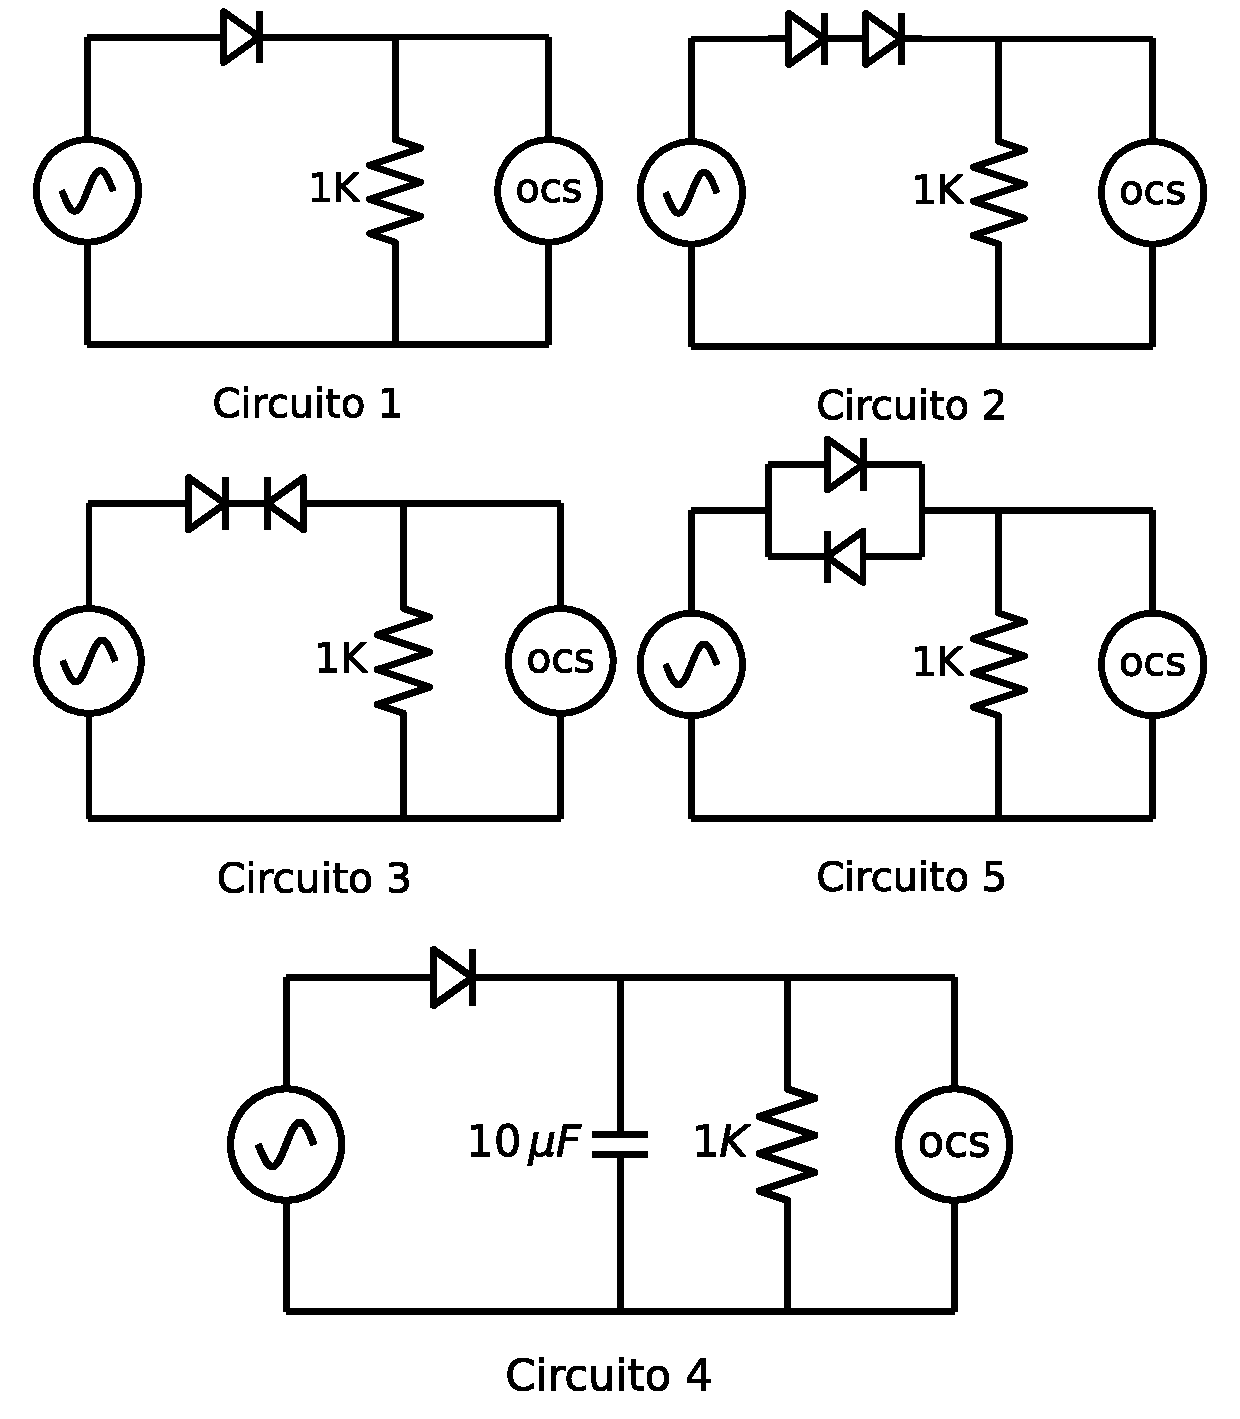
\includegraphics[width=7cm]{imagens/FigB.pdf}
    \caption{Circuitos do procedimento B}
    \label{fig:CircB}
\end{figure}

\section{RESULTADOS EXPERIMENTAIS}

\noindent\textit{A. Curva característica $I_D\times V_D$.}

Ao realizar a parte A do procedimento obtivemos os dados necessários para levantar a curva característica do diodo. Os dados estão relatados na tabela I e a curva característica pode ser vista na figura 3.

\vspace{-.25cm}

\begin{table}[htbp]
    \centering
    \caption{MEDIDAS OBTIDAS PARA OBTER A CURVA}
    \label{tab:medidas}
    \vspace{0.25cm}
    \begin{tabular}{ccc}
        \hline
        \rule{0pt}{3ex} $ V_D \,\,[V]$ & & $ I_D \,\, [mA]$ \\[5pt]
        \hline
        \rule{0pt}{3ex}-0.8 & & 0 \\
        -0.7 & & 0 \\
        -0.6 & & 0 \\
        -0.5 & & 0 \\
        -0.4 & & 0 \\
        -0.3 & & 0 \\
        -0.2 & & 0 \\
        -0.1 & & 0 \\
        0 & & 0 \\
        0.1 & & 0 \\
        0.2 & & 0 \\
        0.3 & & 0 \\
        0.4 & & 0 \\
        0.5 & & 0.7 \\
        0.6 & & 3.3 \\
        0.7 & & 29.7 \\
        0.77 & & 30.4 \\[5pt]
        \hline
    \end{tabular}
\end{table}

\begin{figure}[h]
    \centering
    \includegraphics[width=8cm]{imagens/grafico_ID_x_VD.png}
    \caption{Curva característica $I_D\times V_D$}
    \label{fig:CircA}
\end{figure}

\noindent\textit{B. Análise de Circuitos com diodos BY127.}

\hspace{1cm} Ao realizar a parte B do procedimento obtivemos as curvas de tensão entrada e de saída para cada circuito, anotando a atenuação e defasagem de cada um na tabela II.

\vspace{-.25cm}

\begin{figure}[h]
    \centering
    \includegraphics[width=7cm]{fotos/1.jpg}
    \caption{Circuitos do procedimento B}
    \label{fig:circ1}
\end{figure}

\begin{figure}[h]
    \centering
    \includegraphics[width=7cm]{fotos/1.jpg}
    \caption{Circuitos do procedimento B}
    \label{fig:circ2}
\end{figure}

\begin{figure}[h]
    \centering
    \includegraphics[width=7cm]{fotos/1.jpg}
    \caption{Circuitos do procedimento B}
    \label{fig:circ3}
\end{figure}

\begin{figure}[h]
    \centering
    \includegraphics[width=7cm]{fotos/1.jpg}
    \caption{Circuitos do procedimento B}
    \label{fig:circ4}
\end{figure}

\begin{figure}[h]
    \centering
    \includegraphics[width=7cm]{fotos/1.jpg}
    \caption{Circuitos do procedimento B}
    \label{fig:circ5}
\end{figure}

\begin{table}[htbp]
    \centering
    \caption{DEFASAGEM E ATENUAç ãO DOS CIRCUITOS}
    \label{tab:defasagem}
    \vspace{0.25cm}
    \begin{tabular}{ccc}
        \hline
        \rule{0pt}{3ex}\textbf{Circuito} & \textbf{Defasagem} [ms] & \textbf{Atenuação} [V]\\[5pt]
        \hline
        \rule{0pt}{3ex} 1 &  & \\
        2 &  & \\
        3 & - & - \\
        4 &  & \\
        5 &  & \\[5pt]
        \hline
    \end{tabular}
\end{table}

\section{ANALISE DOS RESULTADOS EXPERIMENTAIS}

\noindent\textit{A. Curva característica do diodo BY127.}

\hspace{1cm} A partir das medidas presentes na tabela (I) e da curva mostrada na figura (3) vemos que o diodo, quando polarizado positivamente, exige uma tensão maior que 0,6 V para conduzir corrente pelo seu ramo. Além disso para valores de tensão VD menor que 0, ou seja polarizado negativamente, o diodo não permitiu passagem de corrente. Isso está de acordo com o datasheet do diodo BY127 [3] em que a tensão de corte está entre 0,6 e 0,8 V, além de que na polarização reversa é esperado que haja pouca, ou quase nenhuma, corrente de saída.

\noindent\textit{B. Análise de Circuitos com diodos BY127.}

\hspace{1cm} Na segunda parte experimental podemos observar pela tabela (II) o diodo real pode ser visto como um diodo perfeito em série com uma queda de tensão, visto que há uma atenuação da tensão de saída. 

\hspace{1cm} Na figura (4) vemos que o circuito funciona como um retificador de meia onda, visto que o diodo não permite a passagem da tensão de entrada quando assume valores negativos. Na figura (5) vemos um aumento da atenuação justificado pelos diodos em série e suas espectivas quedas de tensão. 

\hspace{1cm} Na (6) vemos que os diodos estão com polarização trocada, assim independente da tensão da fonte os diodos funcionarão como circuito aberto. Ao contrário do caso (8) em que os diodos estão em paralelo então, observando a figura (2) o diodo de cima permitirá passagem de corrente para polarização direta, e o diodo de baixo permitirá passagem para polarização reversa.

\hspace{1cm} Por fim, a situação (7) é um caso especial de retificador com capacitor de filtro, ou retificador de pico em que sendo $V_in$, $V_out$, $V_t$ as tensões de entrada, saída e tensão de queda do diodorespectivamente, teremos dois comportamentos de $V_out$ Primeiramente $V_in > V_out$ e o diodo conduz corrente e carrega o capacitor até o valor de pico da entrada. Após, o diodo abre o circuito e apenas o capacitor passa a fornecer tensão para a resistência de forma que $V_out = V_in.e^{-t/RC}$. Por fim, quando a tensão de saída volta aos valores de $V_out < V_in$ o circuito volta para o primeiro estágio.

\section{Conclusão}

\hspace{1cm} Com os resultados e sua conseguinte análise foi possível estudar não só a curva característica de diodos semicondutores para polarização direta e reversa, mas também ficou claro a variadade de usos que o diodo trás pro circuito, principalmente quando utiliza-se o seu comportamento retificador para modificar a saída do circuito. Por fim, os resultados foram congruentes com a teoria estudada.

\section{REFERENCIAS BIBLIOGRAFICAS}

{\small
\begin{enumerate}

    \item CESCHIN, Artemis M. Apostila de materiais eletricos e magneticos.

    \item REZENDE, Sergio M. Materiais e Dispositivos Eletrônicos. 2ª ed. São Paulo: Editora Livraria da Física, 2004.

    \item VISHAY, Miniature Glass Passivated Junction Rectifier, BY127MGP datasheet, 12/03/2012.
    
\end{enumerate}
}

\end{document}